\section{Trabajos relacionados}

\begin{frame}
\frametitle{Antecedentes}
\begin{block}{Opciones de accesibilidad de Microsoft Windows
 \cite{DanielHubbell2016}}
\begin{columns}[T]
\begin{column}{.5\textwidth}

	\begin{itemize}
		\item Lupa.
		\item Narrador.
		\item Teclado en pantalla.
		\item Contraste alto.
		\item Reconocimiento de voz.
	\end{itemize}
\end{column}
\begin{column}{.5\textwidth}
	\begin{figure}[h]
	\centering
	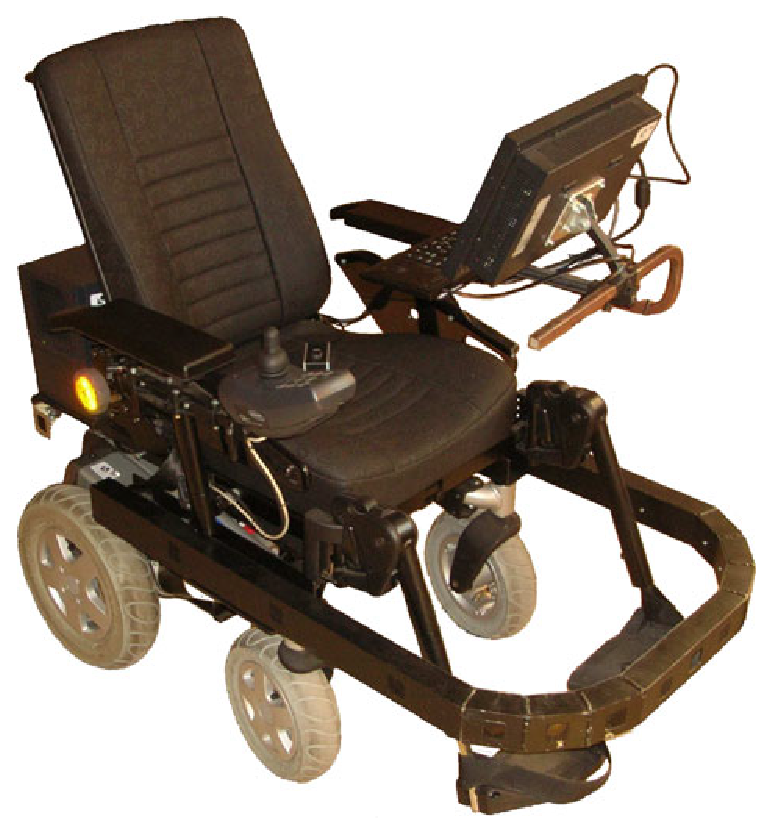
\includegraphics[width=0.6 \columnwidth]{Imagenes/Silla.eps}
	\label{fig:silla}
	\end{figure}
\end{column}
\end{columns}
\end{block}

\begin{block}{Silla de ruedas VAHM3 \cite{Grasse2010}}

\end{block}
\end{frame}

\begin{frame}
\frametitle{Trabajos relacionados}

\begin{table}[!h]
\centering
\scalebox{0.65}{
\begin{tabular}{|p{3.5cm} || p{3.5cm} | p{3.5cm} | p{2.25cm} | p{2cm}|}
\hline

\textbf{Nombre del autor o del proyecto (A\~no)}
& \textbf{interacci\'on con todos los programas del usuario}
& \textbf{Metodolog\'ia empleada}
& \textbf{Automatizar acciones}
& \textbf{M\'ultiples tareas objetivo}
\\ 
\hline
\hline


\textbf{Microsoft Cortana\cite{support17214}(2014)}
& Solo de Microsoft
& Patentado
& Si
& Si
\\ 
\hline

\textbf{Archivo por lotes\cite{Silberschatz1999}(1960)}
& Solo el Sistema Operativo
& Scripts
& Si
& Si
\\ 
\hline

\textbf{Pulover's Macro Creator\cite{Batista}(2013)}
& Si
& Scripts
& Si
& Si
\\ 
\hline

\textbf{UIPath\cite{Dines2018}(2005)}
& Si
& Robotic Process Automation
& Si
& Si
\\
\hline

\textbf{\emph{Propuesta}}
& \textbf{\emph{Si}}
& \textbf{\emph{Grafo}}
& \textbf{\emph{Si}}
& \textbf{\emph{Si}}
\\ 
\hline

\end{tabular}
}
\caption{Tabla de requisitos y an\'alisis comparativo}
\label{ComparativaT}
\end{table}
\end{frame} 